% oss-plantilla: oss-2026.11
% Preámbulo corporativo fijo. No editar en sd-NN.tex: exportar_latex.py verificar lo compara byte a byte.
% Para cambiar el formato, editar esta plantilla u oss.sty y subir la versión de la primera línea.
\PassOptionsToPackage{unicode}{hyperref}
\PassOptionsToPackage{hyphens}{url}
\documentclass[11pt]{article}
\usepackage{amsmath,amssymb}
\usepackage{iftex}
\ifPDFTeX
  % Prism y otros editores en la nube: pdfLaTeX con Helvetica como familia por defecto.
  \usepackage[T1]{fontenc}
  \usepackage[utf8]{inputenc}
  \usepackage{textcomp}
  \usepackage[scaled=0.92]{helvet}
  \renewcommand{\familydefault}{\sfdefault}
  \DeclareUnicodeCharacter{2264}{\ensuremath{\leq}}
  \DeclareUnicodeCharacter{2265}{\ensuremath{\geq}}
  \DeclareUnicodeCharacter{2260}{\ensuremath{\neq}}
  \DeclareUnicodeCharacter{2248}{\ensuremath{\approx}}
  \DeclareUnicodeCharacter{2190}{\ensuremath{\leftarrow}}
  \DeclareUnicodeCharacter{2192}{\ensuremath{\rightarrow}}
  \DeclareUnicodeCharacter{25CF}{\ensuremath{\bullet}}
  \DeclareUnicodeCharacter{2713}{\ensuremath{\checkmark}}
\else
  % XeLaTeX/LuaLaTeX (compilación oficial local): DejaVu Sans.
  \usepackage{fontspec}
  \defaultfontfeatures{Ligatures=TeX,Scale=MatchLowercase}
  \setmainfont{DejaVu Sans}
  \setsansfont{DejaVu Sans}
  \setmonofont{DejaVu Sans Mono}
\fi
\usepackage[letterpaper,margin=20mm]{geometry}
\usepackage{microtype}
\usepackage{parskip}
\usepackage{xcolor}
\usepackage{longtable,booktabs,array}
\usepackage{calc}
\usepackage{etoolbox}
\makeatletter
\patchcmd\longtable{\par}{\if@noskipsec\mbox{}\fi\par}{}{}
\makeatother
\usepackage{footnotehyper}
\makesavenoteenv{longtable}
\usepackage{graphicx}
\makeatletter
\newsavebox\pandoc@box
\newcommand*\pandocbounded[1]{%
  \sbox\pandoc@box{#1}%
  \Gscale@div\@tempa{\textheight}{\dimexpr\ht\pandoc@box+\dp\pandoc@box\relax}%
  \Gscale@div\@tempb{\linewidth}{\wd\pandoc@box}%
  \ifdim\@tempb\p@<\@tempa\p@\let\@tempa\@tempb\fi
  \ifdim\@tempa\p@<\p@\scalebox{\@tempa}{\usebox\pandoc@box}%
  \else\usebox{\pandoc@box}%
  \fi}
\def\maxwidth{\ifdim\Gin@nat@width>\linewidth\linewidth\else\Gin@nat@width\fi}
\def\maxheight{\ifdim\Gin@nat@height>\textheight\textheight\else\Gin@nat@height\fi}
\makeatother
\setkeys{Gin}{width=\maxwidth,height=\maxheight,keepaspectratio}
\makeatletter
\def\fps@figure{htbp}
\makeatother
\usepackage[normalem]{ulem}
\providecommand{\st}[1]{\sout{#1}}
\usepackage{fancyvrb}
\setlength{\emergencystretch}{3em}
\providecommand{\tightlist}{%
  \setlength{\itemsep}{0pt}\setlength{\parskip}{0pt}}
\providecommand{\passthrough}[1]{#1}
\setcounter{secnumdepth}{-\maxdimen}
\ifPDFTeX
  \usepackage[spanish]{babel}
\else
  \usepackage[bidi=default]{babel}
  \babelprovide[main,import]{spanish}
\fi
\let\LanguageShortHands\languageshorthands
\def\languageshorthands#1{}
\usepackage{bookmark}
\usepackage{xurl}
\urlstyle{same}
\hypersetup{pdflang={es-CL},pdfcreator={Only Simple Solutions - exportar_latex.py}}
\usepackage{oss}
\begin{document}

\ossCover{Arquitectura lógica y física de la solución}{Subdocumento 4}
\tableofcontents
\clearpage

\section{Capítulo 4 · Arquitectura lógica y física de la solución}

Este capítulo convierte las responsabilidades y recorridos de SD-03 en componentes desplegables, contratos, datos y emplazamientos. La arquitectura lógica distingue los servicios propios de las plataformas que permanecen; la arquitectura física sitúa los nuevos componentes en nube, centro de datos y tiendas. Las ubicaciones de los sistemas existentes que el Caso no acredita se declaran pendientes de levantamiento, en lugar de atribuirles un alojamiento supuesto. Las especificaciones detalladas de implementos se trazan al Formulario T-11 y las de datos a SD-05.

\section{4.1 Arquitectura lógica}

Esta sección desarrolla el escenario B seleccionado en 3.3 mediante las vistas lógica, de procesos, de despliegue, de datos y de seguridad exigidas por RT-02.03. Los trece servicios de SD-03 describen responsabilidades de negocio; esta sección identifica qué funciones nuevas pueden constituir unidades desplegables y qué plataformas existentes conservan su operación. El número de servicios de negocio no fija el número de procesos ni sustituye las plataformas conservadas. La arquitectura física de 4.2 asigna los componentes nuevos a nube o instalaciones del Cliente y mantiene por verificar el alojamiento individual de las plataformas existentes. No se agregan sistemas para completar el recuento incierto de nueve plataformas del Caso 09.

La Figura 4.1 sitúa los canales, la puerta de enlace, los componentes propios de Retail y del Emisor, el intermediario de eventos por seleccionar, los adaptadores y las plataformas conservadas. Las flechas representan familias de interacción lógica, no las catorce interfaces actuales ni rutas físicas. El asterisco indica que comercio electrónico y fidelización se integran inicialmente y su destino se resuelve mediante pruebas de la primera etapa.

\begin{center}
  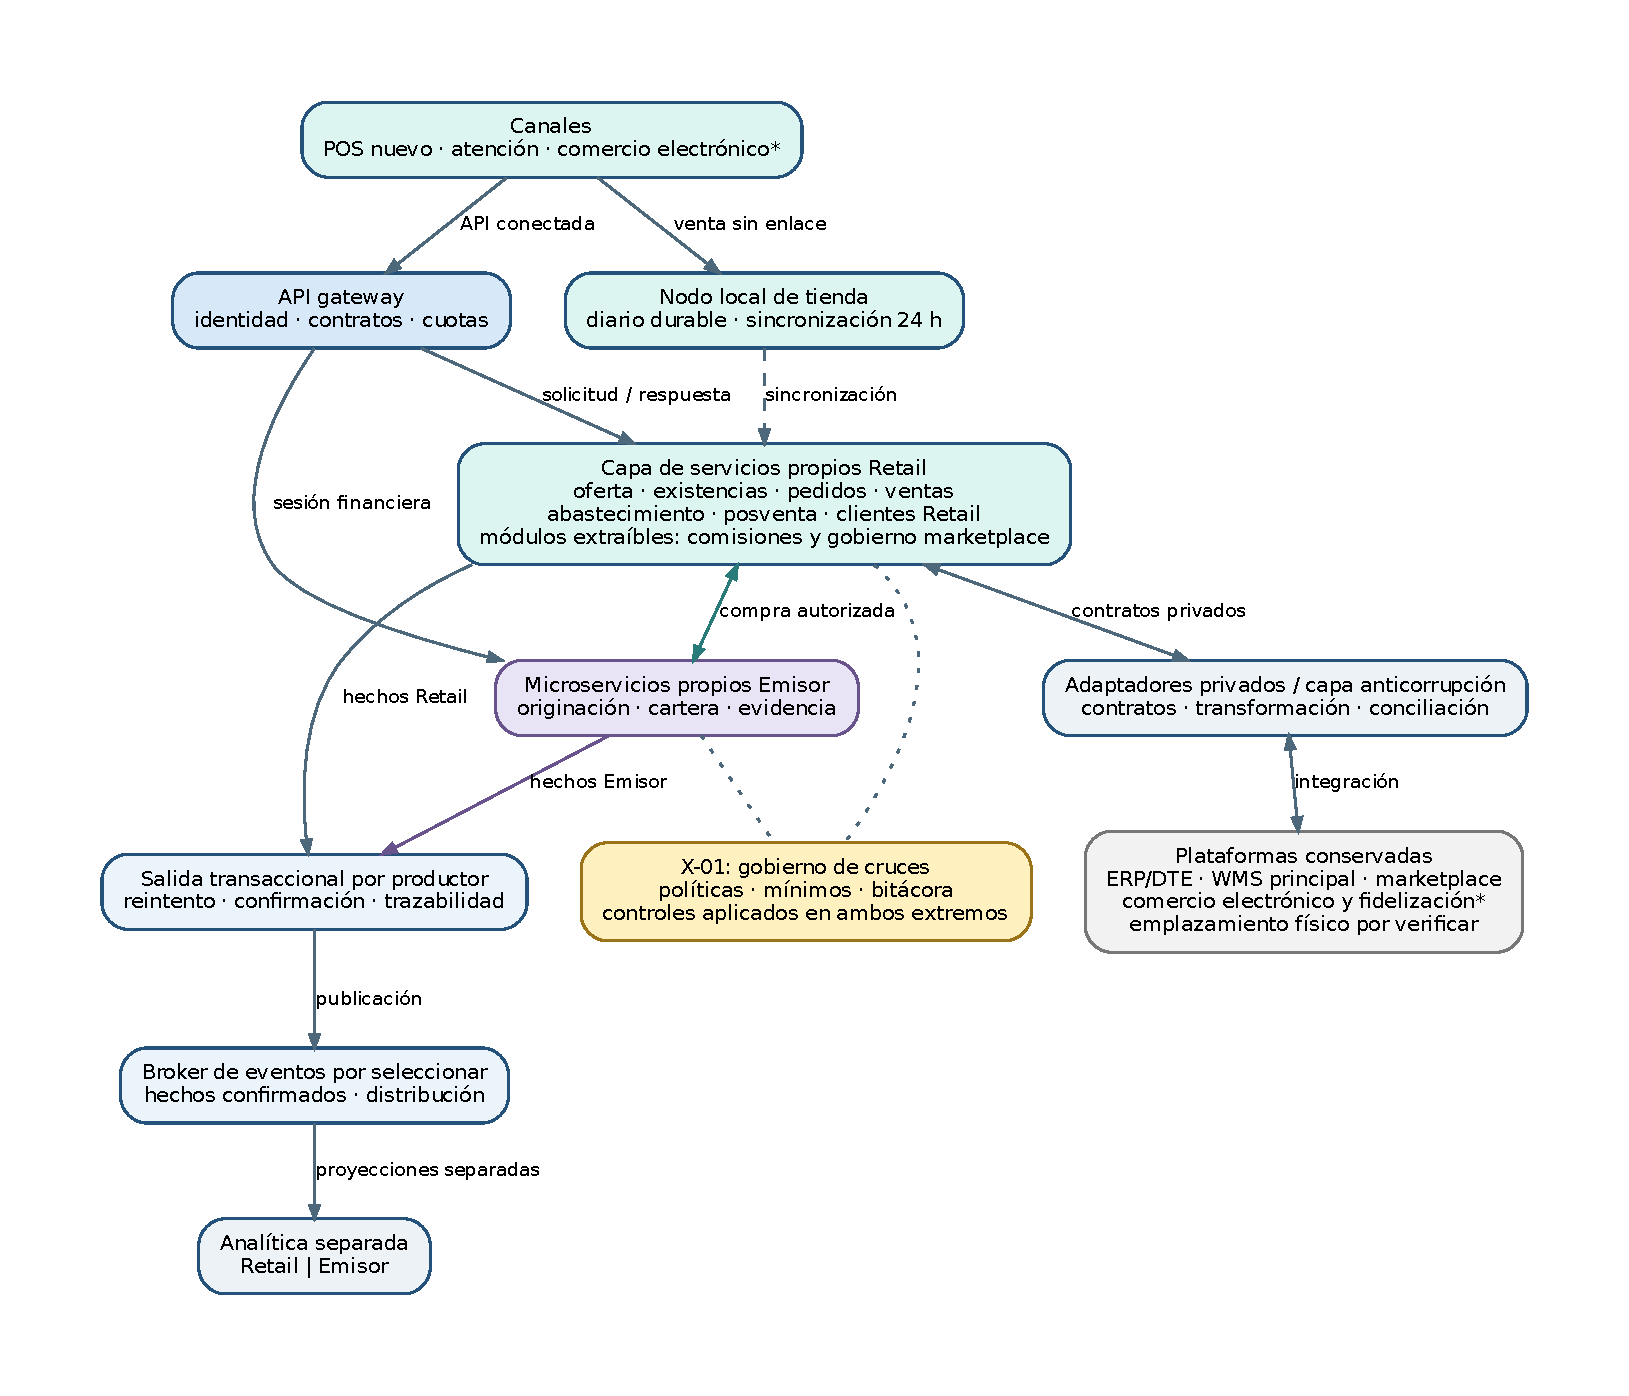
\includegraphics[width=\linewidth]{figuras/diag-04-01_arquitectura-logica.pdf}
\end{center}

Figura 4.1: Ámbitos y relaciones de la arquitectura lógica. Fuente: elaboración propia a partir de SD-03 y del Caso 09.

La figura mantiene Retail y la Filial emisora como autoridades distintas. La línea directa entre ambos representa el contrato de compra condicionado; las líneas punteadas hacia X-01 indican que los extremos aplican su política, sin convertirlo en un repositorio de datos ni en un punto físico de paso obligatorio. «Plataforma conservada» significa externa al límite de los nuevos servicios, no alojada necesariamente en una nube ajena. La filial es una entidad con autoridad propia, no una sede física adicional acreditada por el Caso.

\subsubsection{Vistas y actores de la solución}

La vista lógica identifica las ocho capas de RT-02.01 y los límites Retail, Emisor y Frontera. La vista de procesos sigue venta, pedido, crédito, corte de enlace y recuperación; distingue respuesta síncrona, hecho confirmado y operación local. La vista de despliegue asigna los nuevos componentes a tienda o nube y deja abierta la ubicación individual de los sistemas vigentes. La vista de datos muestra autoridades, proyecciones analíticas y lagos separados. La vista de seguridad muestra identidad, controles en los dos extremos del cruce y auditoría. Estas vistas comparten los códigos de SD-03 para que una misma responsabilidad no cambie de nombre entre diagramas.

La Tabla 4.1 agrupa los treinta y un actores del análisis UAW por entrada y ámbito. Es un mapa de cobertura, no una nueva estimación de puntos de caso de uso. AH-17 utiliza una API por decisión del equipo; AS-11 representa el módulo de remuneraciones de AS-01 y AS-14 un disparador periódico. AS-06 no figura en el catálogo aportado. Una interfaz objetivo no demuestra que la API exista hoy ni que la plataforma esté alojada en el centro de datos de casa matriz.

Tabla 4.1: Grupos de actores, entrada y destino lógico.

\begin{longtable}{@{}p{0.25\linewidth}p{0.31\linewidth}p{0.36\linewidth}@{}}
\toprule Actores UAW & Canal o contrato & Destino responsable \\
\midrule\endhead\bottomrule\endlastfoot
AH-01, AH-03, AH-04 & Comercio electrónico, terminal compartida y POS. & Oferta, existencias, pedidos y ventas Retail; sesión financiera separada cuando corresponde. \\
AH-05, AH-06, AH-08, AH-14 & Terminal de conteo, reposición, exhibición y prevención. & Existencias y oferta; modelos de merma solo proponen causas. \\
AH-07 & Vista logística en ambos centros de distribución. & Abastecimiento, existencias y pedidos; WMS solo en el centro principal. \\
AH-09, AH-11, AH-12, AH-13 & Atención, consola comercial y planificación. & Posventa, oferta, abastecimiento, clientes Retail y gobierno marketplace. \\
AH-02, AH-10 & Acceso del titular y puesto financiero. & Originación, cartera y evidencia del Emisor. \\
AH-15, AH-16, AH-18 & Auditoría, operación y autoservicio BI. & X-01, seguridad/telemetría y analítica separada según rol. \\
AH-17 & API de vendedor externo. & Gobierno marketplace por gateway y contrato autorizado. \\
AS-01 a AS-05, AS-11 & Adaptadores ERP/DTE, WMS, marketplace, canal digital y fidelización. & Interfaces de conservación; AS-11 es remuneraciones de AS-01. \\
AS-07, AS-08, AS-12, AS-13 & Contratos de transportista, pago, fiscalización y proveedor. & Pedidos, ventas, reportes del Emisor y abastecimiento según finalidad. \\
AS-09, AS-10, AS-14 & Archivos de convivencia y temporizador. & Migración Retail/Emisor y disparo de conciliaciones; sin autoridad nueva. \\
\end{longtable}

La tabla conserva todos los códigos AH-01 a AH-18 y AS-01 a AS-14 salvo AS-06, ausente en el registro UAW. El cliente, el titular de tarjeta y el ejecutivo financiero pueden compartir una instalación física sin compartir datos ni permisos. La Figura 4.2 amplía las capas y entradas por ámbito; su fuente editable mantiene la correspondencia de códigos para el diagrama final.

\begin{center}
  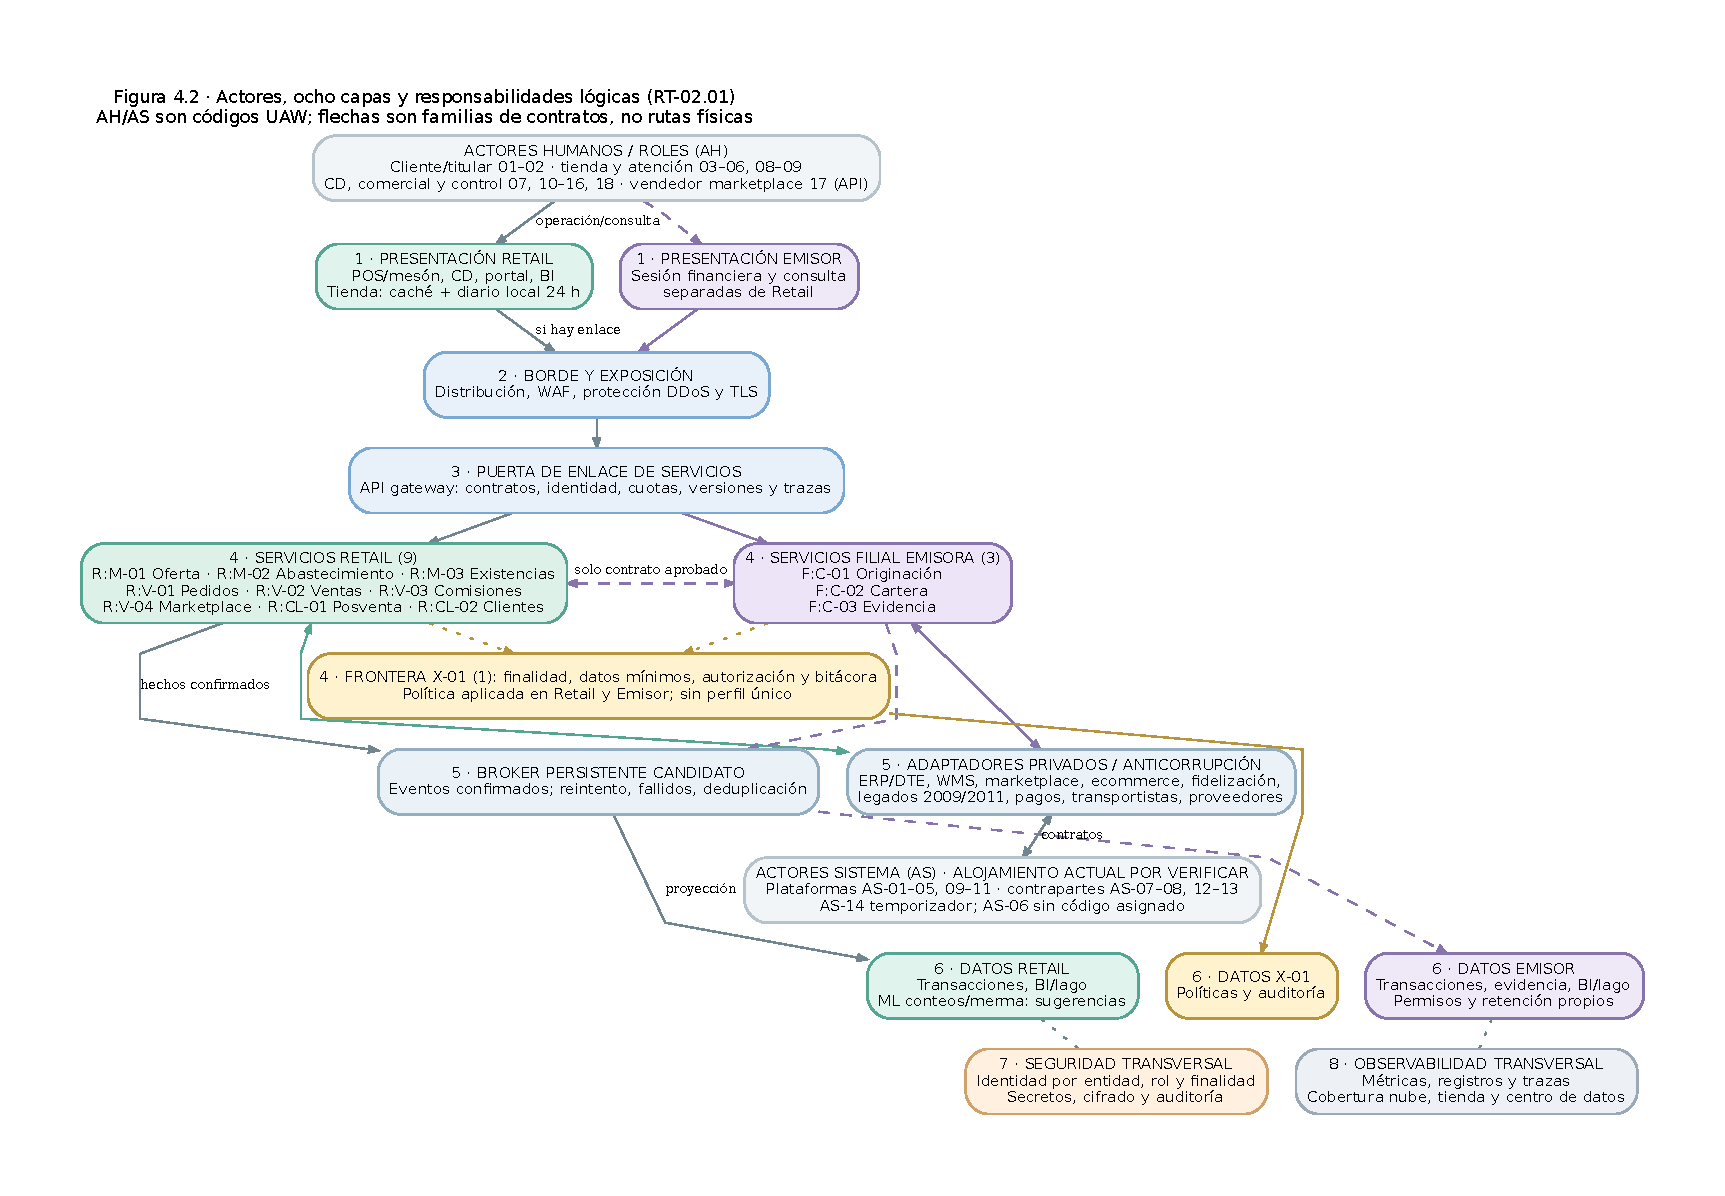
\includegraphics[width=\linewidth]{figuras/diag-04-02_capas-y-actores.pdf}
\end{center}

Figura 4.2: Actores, ocho capas y servicios por ámbito. Fuente: elaboración propia a partir de SD-03, Bases Transversales RT-02.01 y catálogo UAW aportado.

En la figura, seguridad y observabilidad atraviesan las demás capas. Los actores de sistemas se conectan por contratos o adaptadores; ninguno obtiene acceso directo a la base de datos de un servicio nuevo. Los trece códigos R/F/X identifican autoridad funcional y no trece despliegues obligatorios.

\subsubsection{Estilo y límites de contexto}

La solución separa tres frentes: Retail, Filial emisora y Frontera. Retail contiene las áreas Mercadería, Venta y Relación con el cliente; la Filial emisora contiene Crédito. El Servicio de control de cruces X-01 gobierna el intercambio entre entidades, sin hacerse dueño de sus datos. La plataforma común proporciona identidad, contratos, transporte, adaptadores y observabilidad. Su papel es habilitar los flujos, no concentrar las reglas de negocio ni actuar como un maestro único de clientes.

Cada servicio controla la escritura de sus registros y publica solo vistas o hechos necesarios para consumidores autorizados. Una consulta transversal no puede leer directamente la base de otro ámbito. La identidad comercial R:CL-02 y la identidad financiera se vinculan únicamente para finalidades aprobadas por X-01. Saldos, mora, cupos y comportamiento de pago permanecen en Crédito; no se replican al perfil comercial ni a Marketing.

La descomposición aplica contextos delimitados del dominio y conserva juntas las reglas que deben confirmar una transacción. Una unidad se separa como microservicio cuando tiene autoridad de datos clara y necesita evolucionar, escalar o recuperarse de forma independiente. Los módulos de comisiones y gobierno de marketplace pueden permanecer dentro de un despliegue compartido hasta que las mediciones justifiquen extraerlos. Se comparó esta separación selectiva con un despliegue único de todos los módulos: el primero aísla ventas, existencias y crédito, que tienen cargas, autoridades y recuperación distintas; el segundo reduce operación, pero amplía el radio de falla y obliga a desplegarlos juntos. La comparación se completará con volumetría, competencias del equipo y el inventario de interfaces, conforme al capítulo 2 de las Bases Transversales.

\subsubsection{Catálogo de componentes y autoridad}

La Tabla 4.2 asigna a cada servicio su registro principal. Los códigos son identificadores de arquitectura para trazar esta vista con 3.3 y 3.4, no sustituyen los identificadores de requisitos del catálogo.

Tabla 4.2: Servicios y autoridad del dato en la arquitectura lógica.

\begin{longtable}{@{}p{0.15\linewidth}p{0.34\linewidth}p{0.43\linewidth}@{}}
\toprule Código & Servicio & Autoridad y límite \\
\midrule\endhead\bottomrule\endlastfoot
R:M-01 & Servicio de oferta comercial & Artículos, precios, promociones, vigencias y publicación; no reserva existencias. \\
R:M-02 & Servicio de abastecimiento & Órdenes, transferencias y recepción coordinada; WMS conserva la ejecución física. \\
R:M-03 & Servicio de existencias & Movimientos conciliados, conteos, reservas y disponible comprometible; ERP/DTE conserva el asiento contable. \\
R:V-01 & Servicio de pedidos & Estado único, promesa, asignación y seguimiento; no ejecuta la preparación del almacén. \\
R:V-02 & Servicio de ventas & Venta, pago, reversa y conciliación de caja; ERP/DTE es el único emisor tributario. \\
R:V-03 & Servicio de comisiones & Regla y base de atribución; el sistema empresarial conserva remuneraciones. \\
R:V-04 & Servicio de marketplace & Reglas de vendedores y coordinación; se integra con la plataforma vigente. \\
R:CL-01 & Servicio de posventa & Caso y destino de devolución; reintegro al disponible sujeto a inspección. \\
R:CL-02 & Servicio de clientes Retail & Identificación y preferencias; fidelización conserva puntos y campañas durante la convivencia. \\
F:C-01 & Servicio de originación de crédito & Solicitud, evaluación, cupo y autorización; apertura sujeta a evidencia. \\
F:C-02 & Servicio de cartera de crédito & Cuenta, saldo, pago, mora, cobranza y repactación; migración por olas. \\
F:C-03 & Servicio de evidencia financiera & Versiones precontractuales, aceptación, firma y expediente; no decide crédito. \\
X-01 & Servicio de control de cruces & Fichas, políticas, decisiones y bitácora del intercambio; no almacena perfiles unificados. \\
\end{longtable}

La asignación distingue el registro comercial, el registro financiero y las funciones que permanecen en ERP/DTE, WMS y remuneraciones. Esta distinción permite comprobar qué sistema puede aceptar una escritura y qué datos entrega a otros ámbitos.

La Tabla 4.3 traduce los contextos de SD-03 en unidades técnicas candidatas. «Módulo» indica una responsabilidad implementada en el nuevo sistema que aún no necesita un despliegue independiente; «microservicio» indica autoridad y ciclo operativo propios. La partición definitiva se revisará con la latencia, volumetría y esfuerzo de operación, sin modificar por ello el catálogo funcional de trece servicios.

Tabla 4.3: Candidatos de despliegue derivados de los servicios de negocio.

\begin{longtable}{@{}p{0.16\linewidth}p{0.42\linewidth}p{0.34\linewidth}@{}}
\toprule SD-03 & Unidad técnica candidata & Criterio inicial \\
\midrule\endhead\bottomrule\endlastfoot
R:M-01 & Catálogo de artículos; precios, promociones y publicación. & Evaluar dos microservicios por reglas y carga de cambios distintas. \\
R:M-02 & Órdenes y coordinación de reposición. & Una unidad; WMS retiene la ejecución física. \\
R:M-03 & Movimientos, reservas, disponible, conteos y ajustes. & Un microservicio transaccional para preservar la promesa de stock. \\
R:V-01 & Estado, promesa y coordinación de pedidos. & Una unidad; WMS ejecuta preparación y despacho. \\
R:V-02 & Venta, pago, reversa y conciliación. & Un microservicio; POS local es canal y ERP/DTE emite documentos. \\
R:V-03 & Reglas y base de comisiones. & Módulo extraíble; ERP conserva remuneraciones. \\
R:V-04 & Gobierno e intercambio con marketplace. & Módulo extraíble; la plataforma de terceros permanece. \\
R:CL-01 & Expediente de posventa e inspección. & Microservicio por reglas y autoridad del caso. \\
R:CL-02 & Identidad y preferencias comerciales. & Una unidad; puntos y campañas quedan en fidelización durante la convivencia. \\
F:C-01 & Originación, decisión y autorización. & Un microservicio inicial para preservar cupo y plazo de respuesta. \\
F:C-02 & Cartera, pagos, cobranza y repactación. & Microservicio separado por migración y operación. \\
F:C-03 & Evidencia y consentimiento financiero. & Microservicio separado por custodia y retención. \\
X-01 & Gobierno de políticas y bitácora de cruces. & Unidad de gobierno; aplicación de políticas en ambos extremos. \\
\end{longtable}

La predicción de conteos y la clasificación de merma, si superan su validación de datos y beneficio, se ejecutan como procesadores de apoyo de Retail. Producen recomendaciones para R:M-03 y no escriben ajustes ni el disponible comprometible. La capacidad analítica es una plataforma de lectura con espacios separados por ámbito; tampoco se suma al catálogo de servicios de negocio.

\subsubsection{Capas e interfaces}

La presentación incluye comercio electrónico, caja/POS, terminales móviles compartidas, atención, consola logística, acceso financiero, BI y entrada API de vendedor externo. El borde expone contenido y aplica protección perimetral; el API gateway es la entrada de las APIs autorizadas y aplica identidad, cuotas, validación de contratos y trazabilidad. La capa de servicios contiene las unidades propias de Retail, Emisor y Frontera, no las plataformas conservadas. La integración contiene contratos síncronos, publicación durable de hechos confirmados, un broker por seleccionar y adaptadores privados por contraparte. La capa de datos separa repositorios transaccionales, documentos y espacios analíticos por ámbito. Seguridad y observabilidad atraviesan todas las capas. Estas ocho responsabilidades corresponden a RT-02.01. El nodo local de tienda conserva oferta vigente, existencia local y diario durable; el POS separa la función Retail de una eventual sesión financiera bajo rol propio.

La Tabla 4.4 fija el destino de cada plataforma sin inferir su alojamiento. El Caso 09 acredita un centro de datos propio de 140 m², sala de respaldo en la misma comuna y uso compartido de centro y red por Retail y Emisor, pero no asigna individualmente cada sistema a ese centro ni a una nube externa. El inventario de las catorce interfaces y sus ubicaciones precede el retiro de cualquier conexión antigua.

Tabla 4.4: Destino de plataformas actuales y ubicación acreditada.

\begin{longtable}{@{}p{0.27\linewidth}p{0.39\linewidth}p{0.26\linewidth}@{}}
\toprule Plataforma & Destino y responsabilidad retenida & Alojamiento actual \\
\midrule\endhead\bottomrule\endlastfoot
ERP/DTE & Se conserva; contabilidad, remuneraciones y única emisión tributaria. & Por verificar. \\
WMS principal & Se conserva; ubicaciones, preparación y despacho, con extensión a Concepción por evaluar. & Operación en CD principal; servidor por verificar. \\
Marketplace 2022 & Se conserva; plataforma de terceros y liquidaciones. & Por verificar. \\
Comercio electrónico 2019 & Se integra inicialmente; conservación, remediación o sustitución tras pruebas. & Por verificar. \\
Fidelización 2017 & Se integra inicialmente; destino posterior sujeto a pruebas. & Por verificar. \\
Núcleo Retail 2009 & Se reemplaza por olas conciliadas. & Por verificar. \\
Plataforma de crédito 2011 & Se reemplaza por olas de cartera y funciones. & Por verificar. \\
POS de tienda 2014 & Se sustituye tienda por tienda. & Terminales en tienda; dependencias por verificar. \\
Motor de precios & No existe como sistema; se construye capacidad nueva. & No aplica. \\
\end{longtable}

Los adaptadores aíslan los modelos de ERP/DTE, WMS y marketplace y los contratos temporales de comercio electrónico, fidelización, núcleo Retail 2009 y crédito 2011. Cubren asimismo transportistas, medios de pago y proveedores cuando el contrato de cada contraparte lo exija. Cada uno declara autoridad de origen, dirección, frecuencia, versión, confirmación, plazo de respuesta y regla de conciliación. AS-11 identifica la interfaz de remuneraciones dentro del ERP, sin duplicarlo como plataforma. AS-09 y AS-10 usan archivo o protocolo durante la convivencia; AS-13 conserva el medio de intercambio por confirmar. Una API de vendedor marketplace podrá exponerse mediante el gateway; la traducción hacia la plataforma conservada permanece en el adaptador. No se atribuye alojamiento a un sistema por el hecho de conectarlo.

Las solicitudes que necesitan respuesta para continuar, como reserva previa al cobro, autorización de compra o comprobación de evidencia antes de abrir crédito, usan contratos síncronos con plazo máximo, identificador de operación e idempotencia. Los hechos ya confirmados, como venta registrada, movimiento conciliado, pedido cambiado de estado o recepción de devolución, se publican en el intermediario de eventos seleccionado mediante un registro de salida transaccional por productor. Cada hecho incluye versión, clave de agregado y correlación. La entrega es al menos una vez: cada consumidor deduplica, confirma, reintenta y deriva errores persistentes a tratamiento controlado. Cuando un proceso exige orden, se conserva por agregado o partición. Recibir un evento no equivale a aplicar exitosamente su efecto. Kafka es una preferencia del equipo, no una exigencia de las Bases; Event Hubs y Service Bus se comparan por relectura, semántica de entrega, tratamiento de errores y operación híbrida, sin llamar Apache Kafka a un servicio solo compatible con su protocolo.

\subsubsection{Recorridos y consistencia}

La vista de procesos sigue el hecho desde la persona o sistema que lo origina hasta el registro de autoridad, su salida y el consumidor. La Figura 4.3 distingue operación conectada, diario local durante veinticuatro horas sin enlace, retorno conciliado y cruce autorizado con el Emisor. Las flechas continuas son contratos del diseño; las discontinuas representan publicación diferida o rutas que requieren confirmar el enlace.

\begin{center}
  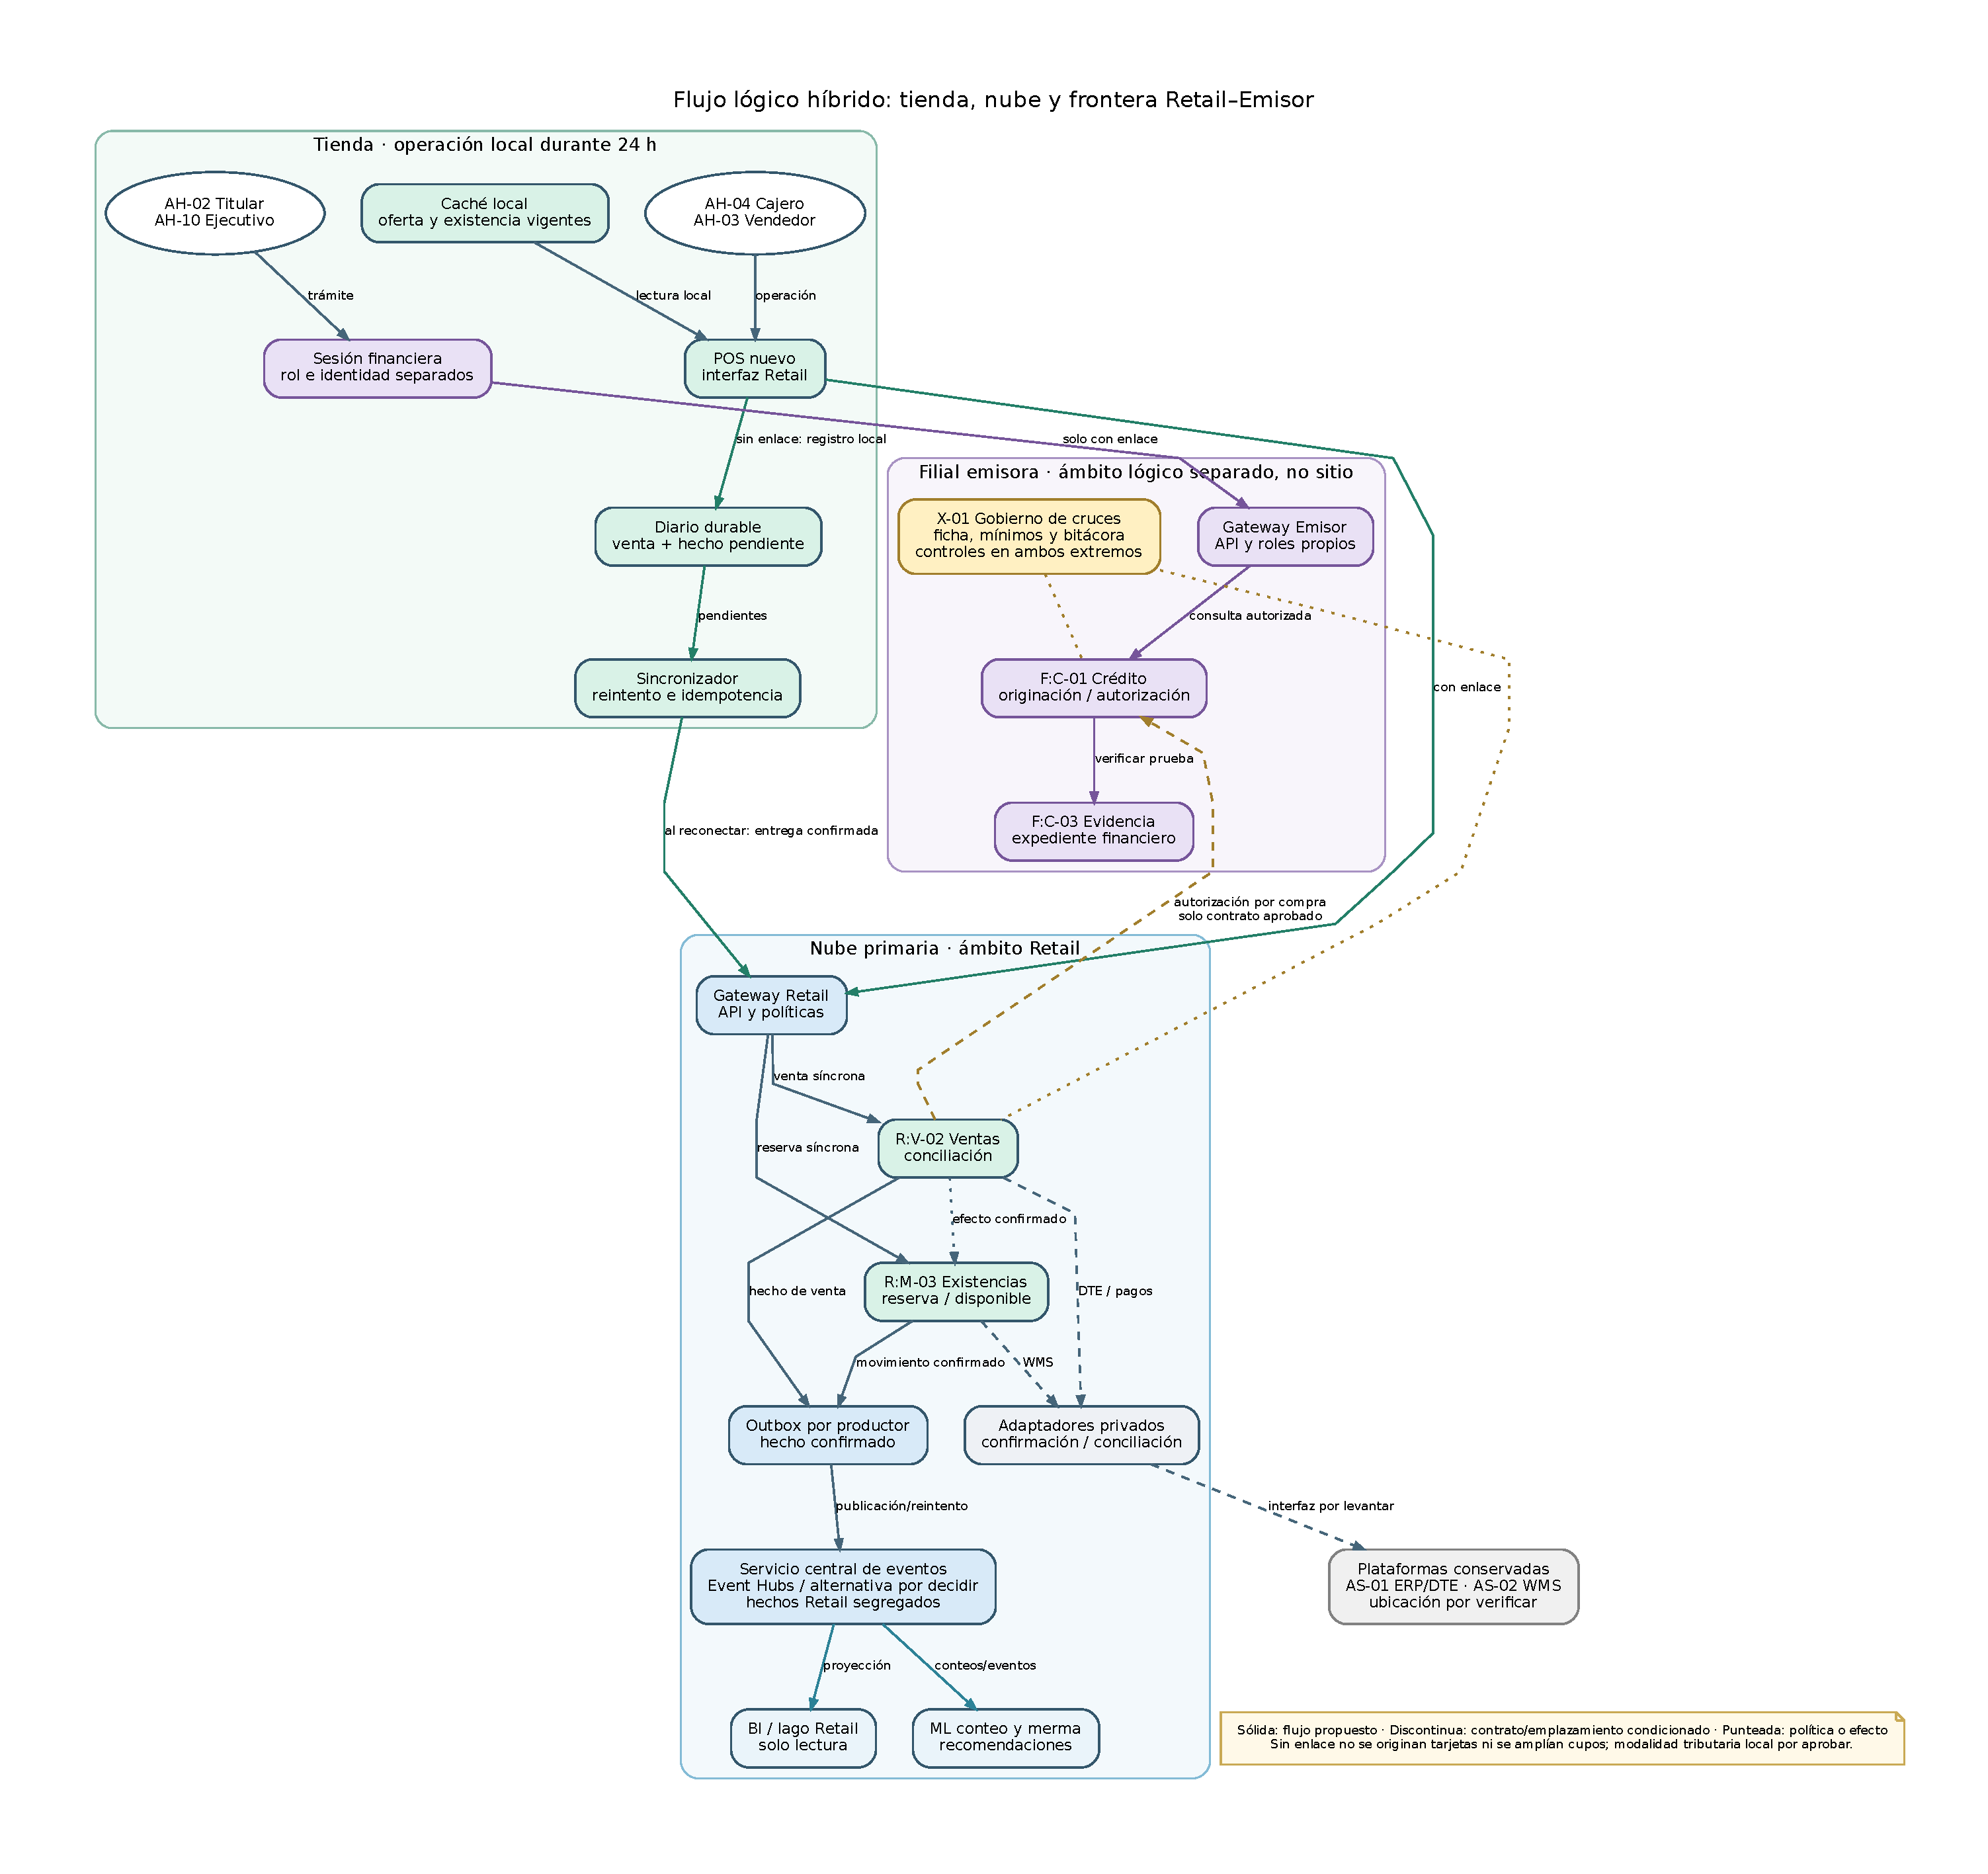
\includegraphics[width=\linewidth]{figuras/diag-04-03_flujo-hibrido.pdf}
\end{center}

Figura 4.3: Flujo híbrido de venta, conciliación, eventos y crédito segregado. Fuente: elaboración propia a partir de SD-03 y RT-02/RT-03.

El POS escribe primero la operación y el hecho pendiente en su diario. Un broker en nube, sea Kafka, Event Hubs o Service Bus, no conserva un evento que aún no recibió por una interrupción WAN. Al volver el enlace, el sincronizador envía con confirmación y clave idempotente a R:V-02; solo tras su conciliación se publica el hecho confirmado. El registro de salida pertenece a cada productor, no es una transacción compartida entre Ventas y Existencias. Un broker en tienda o en el centro de datos se agregará únicamente si el levantamiento demuestra varios consumidores locales que deban intercambiar mientras la nube no está disponible.

\textbf{Existencia y venta.} R:M-01 publica oferta; R:M-03 calcula el disponible comprometible a partir de movimientos conciliados, reservas y margen de confianza por categoría y nodo. R:V-01 solicita y confirma una reserva antes de prometer entrega; R:V-02 registra la venta. Cada reserva tiene vigencia, clave de idempotencia y estados confirmada, liberada o expirada. El canal no cobra si no recibe confirmación de disponibilidad. Una venta se propaga hacia la disponibilidad publicada con el plazo exigido de 30 segundos; retrasos, duplicados y desorden de eventos se detectan por identificador y versión.

\textbf{Precio.} R:M-01 mantiene una versión aprobada de precio y promoción por canal y vigencia. POS y canal digital registran la versión aplicada y la elegibilidad consultada a R:CL-02 cuando procede. Las etiquetas de tienda tienen confirmación de actualización y divergencias registradas. La política comercial ante una diferencia entre etiqueta y caja queda por acordar antes del despliegue; la arquitectura conserva la evidencia necesaria para resolverla.

\textbf{Pedido y devolución.} R:V-01 recibe cambios de estado de tienda, WMS y transportista y conserva la promesa y su historial. R:V-03 calcula la atribución tras la venta confirmada y la ajusta ante reversas. R:CL-01 registra la recepción física, inspección y destino de la devolución; comunica al vendedor externo por R:V-04 y solicita el cambio de disponibilidad a R:M-03 solo cuando la unidad puede venderse de nuevo. ERP/DTE emite el documento tributario o la nota de crédito correspondiente.

\textbf{Crédito y frontera.} F:C-01 y F:C-02 consultan F:C-03 antes de confirmar apertura o repactación. Para una compra con tarjeta propia, R:V-02 envía referencia e importe mediante el contrato habilitado por X-01; F:C-01 devuelve una decisión limitada a esa operación. X-01 versiona la ficha de finalidad, fundamento, campos y responsables y exige controles en los dos extremos. Una consulta de Marketing sobre pago se deniega y audita. Las rutas de reversa y conciliación con F:C-02 permanecen cerradas hasta acreditar necesidad, contrato y aprobación, según la Tabla 3.7. Ni la ausencia de respuesta ni el consentimiento de originación se interpretan como autorización de compra.

\subsubsection{Vista de despliegue lógico y sitios}

La Figura 4.4 separa emplazamientos, autoridades y rutas. SIT-01 agrupa las 22 tiendas: cada una necesita POS, almacenamiento local durable y sincronizador. CD-01 es el centro de distribución principal y CD-02 el de Concepción; ambos son lugares de operación logística, no ubicaciones acreditadas de servidores WMS. DC-01 identifica el centro de datos de casa matriz y DC-02 su sala de respaldo en la misma comuna. CLD-01 y CLD-02 representan la región primaria propuesta y la de recuperación condicionada. EXT-01 agrupa contrapartes externas. La Filial emisora comparte infraestructura acreditada con Retail, pero conserva un dominio lógico y de datos independiente. El broker se propone en CLD-01 y se recupera en CLD-02; un broker adicional en tienda o centro de datos dependerá de una necesidad local medida.

\begin{center}
  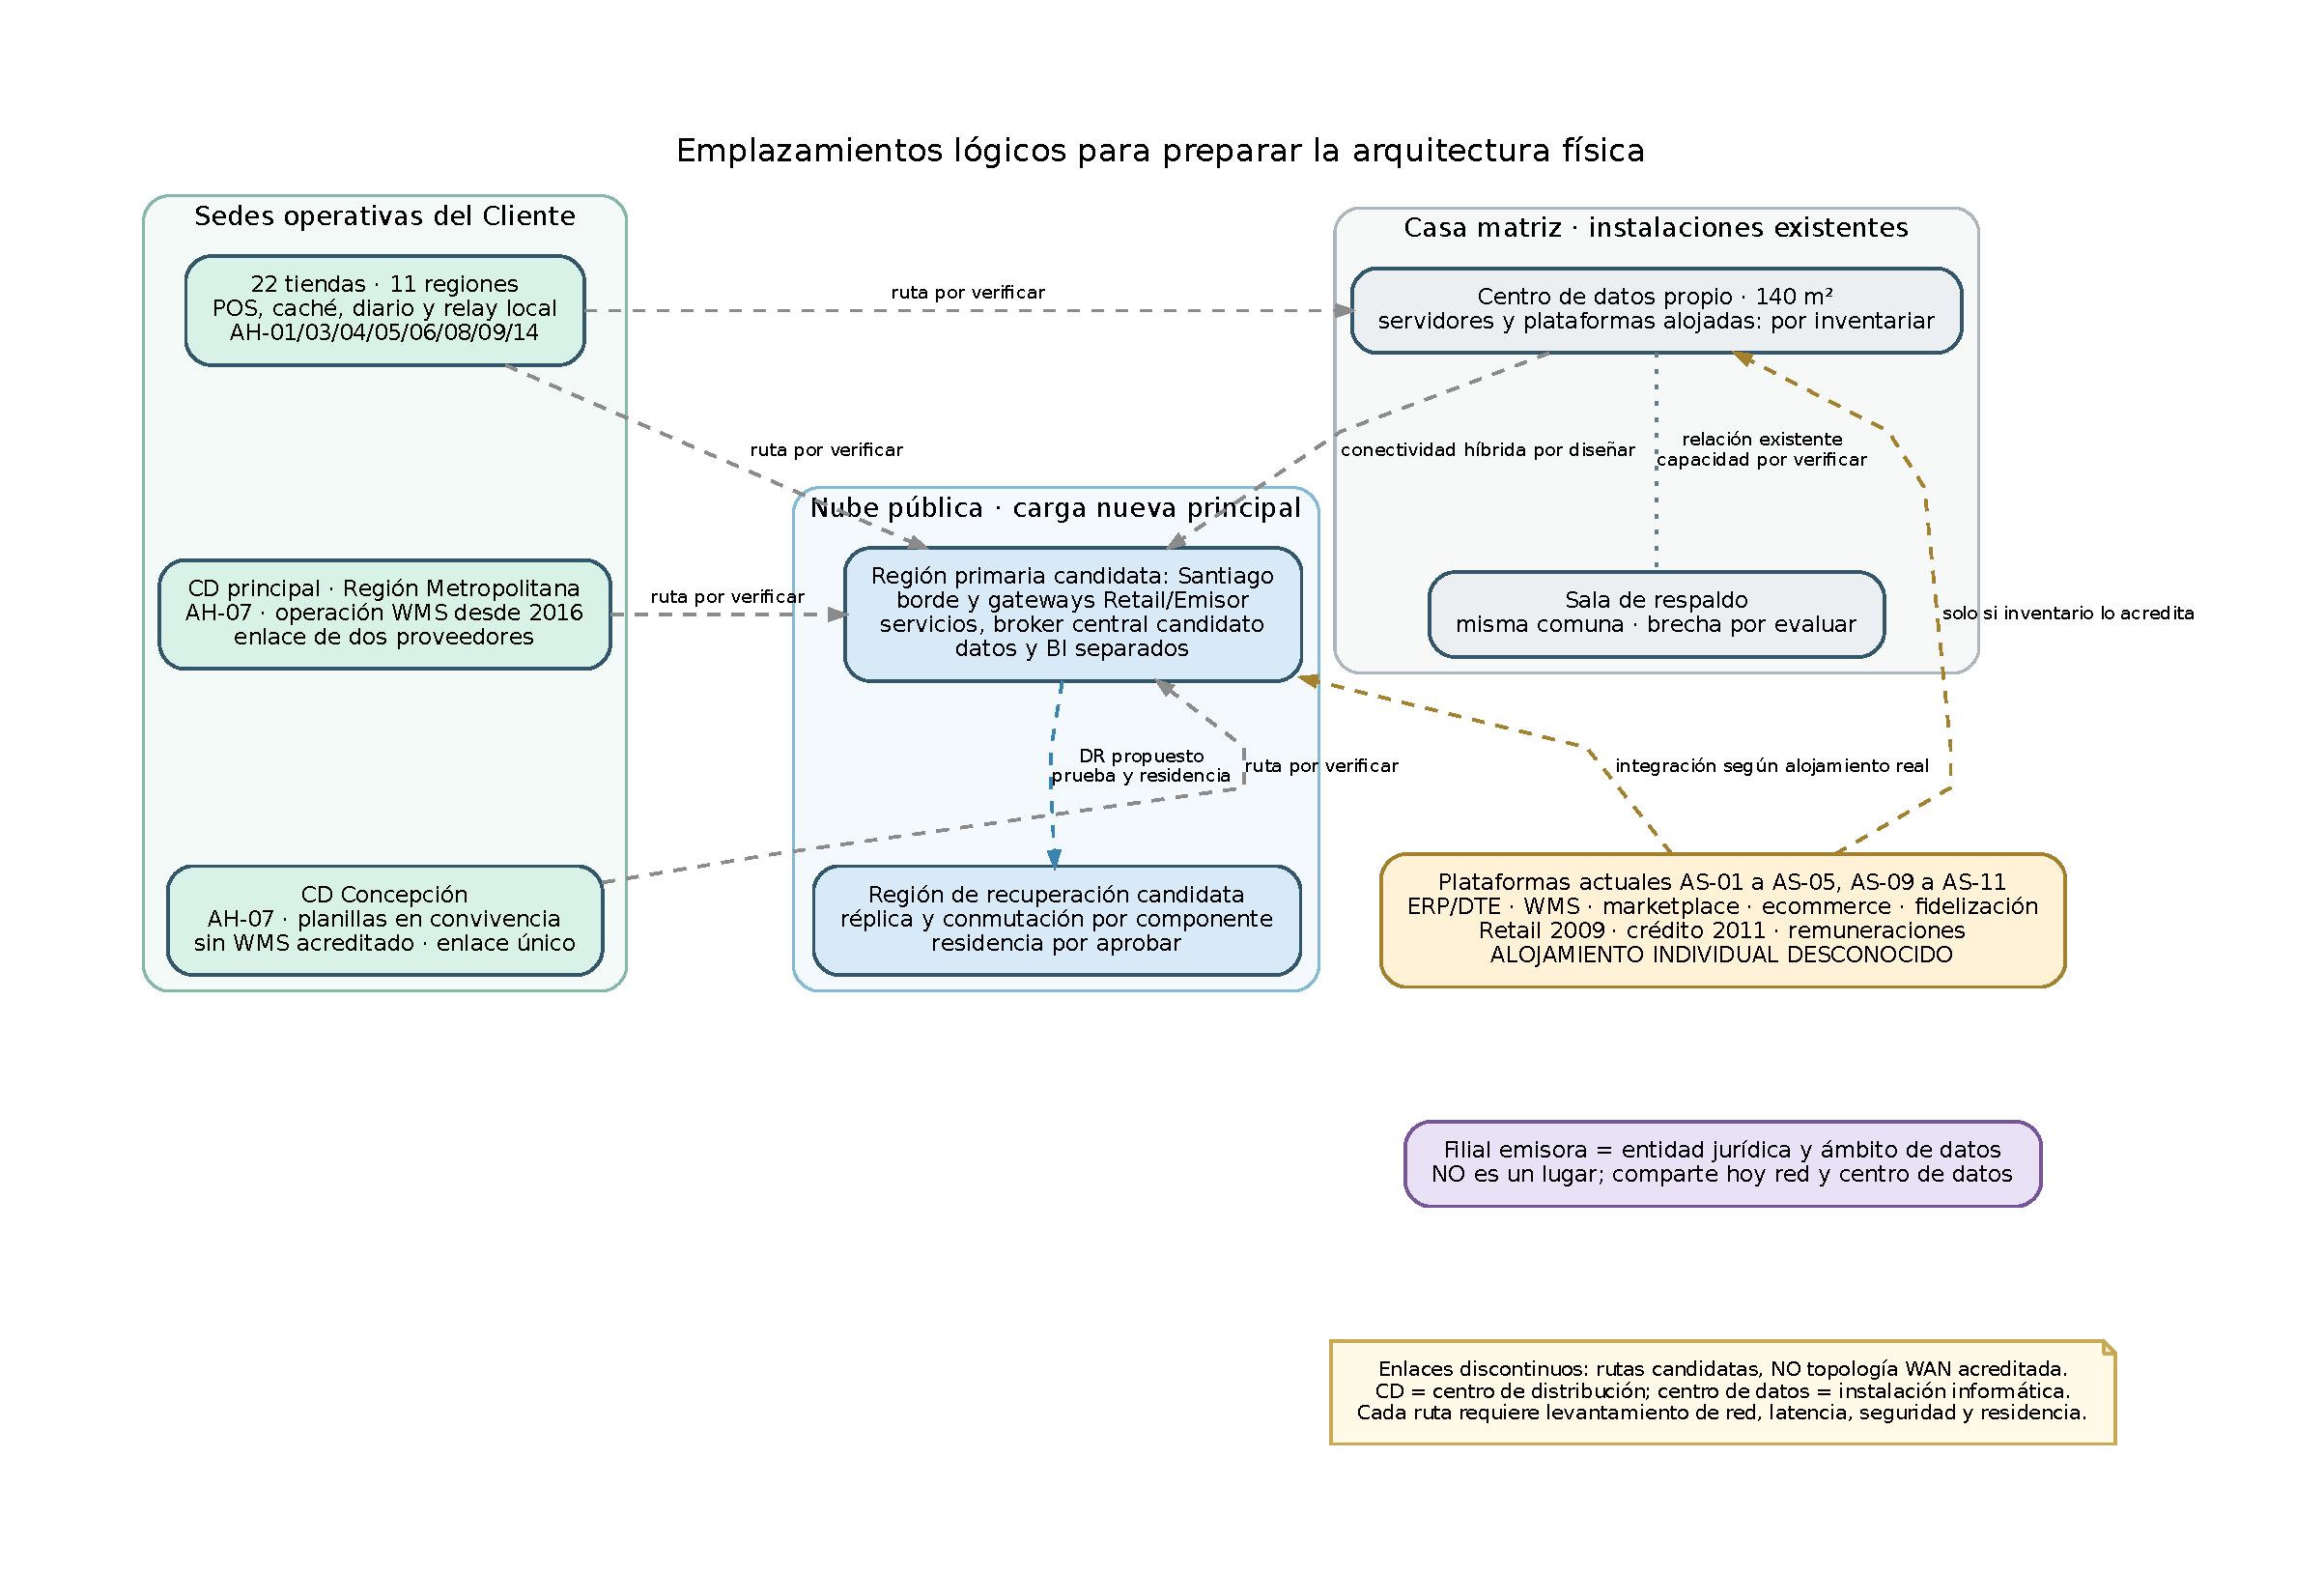
\includegraphics[width=\linewidth]{figuras/diag-04-04_emplazamientos-logicos.pdf}
\end{center}

Figura 4.4: Emplazamientos y rutas lógicas. Fuente: elaboración propia a partir del Caso 09, RT-03 y SD-03.

La conectividad de tienda, centros de distribución y centro de datos con la nube debe inventariarse antes de fijar rutas, redundancia y capacidad. Una flecha hacia una plataforma heredada indica intercambio funcional; el trayecto físico queda por acreditar. La venta sin enlace termina primero en el diario de SIT-01 y se reconcilia al recuperar conectividad. No se presupone que el tráfico de cada tienda pase por CD-01 ni que el WMS esté hospedado allí.

\subsubsection{Vista de datos y seguridad}

La Figura 4.5 sitúa el dato comercial, el financiero y sus proyecciones analíticas en dominios separados. Los lagos y espacios BI son de lectura y mantienen control de acceso, linaje y exportación por entidad. R:CL-02 no recibe mora, saldo ni pagos. La compra con tarjeta cruza únicamente referencia, importe, medio y decisión mínima, con ficha de X-01 aprobada y controles aplicados en los dos extremos. Los modelos de conteo predictivo y clasificación de merma consultan datos autorizados de Retail y entregan recomendaciones para revisión humana; no ajustan existencias por sí mismos. Una proyección analítica que mezcle ámbitos permanece deshabilitada hasta justificar finalidad, minimización y permiso jurídico propios.

\begin{center}
  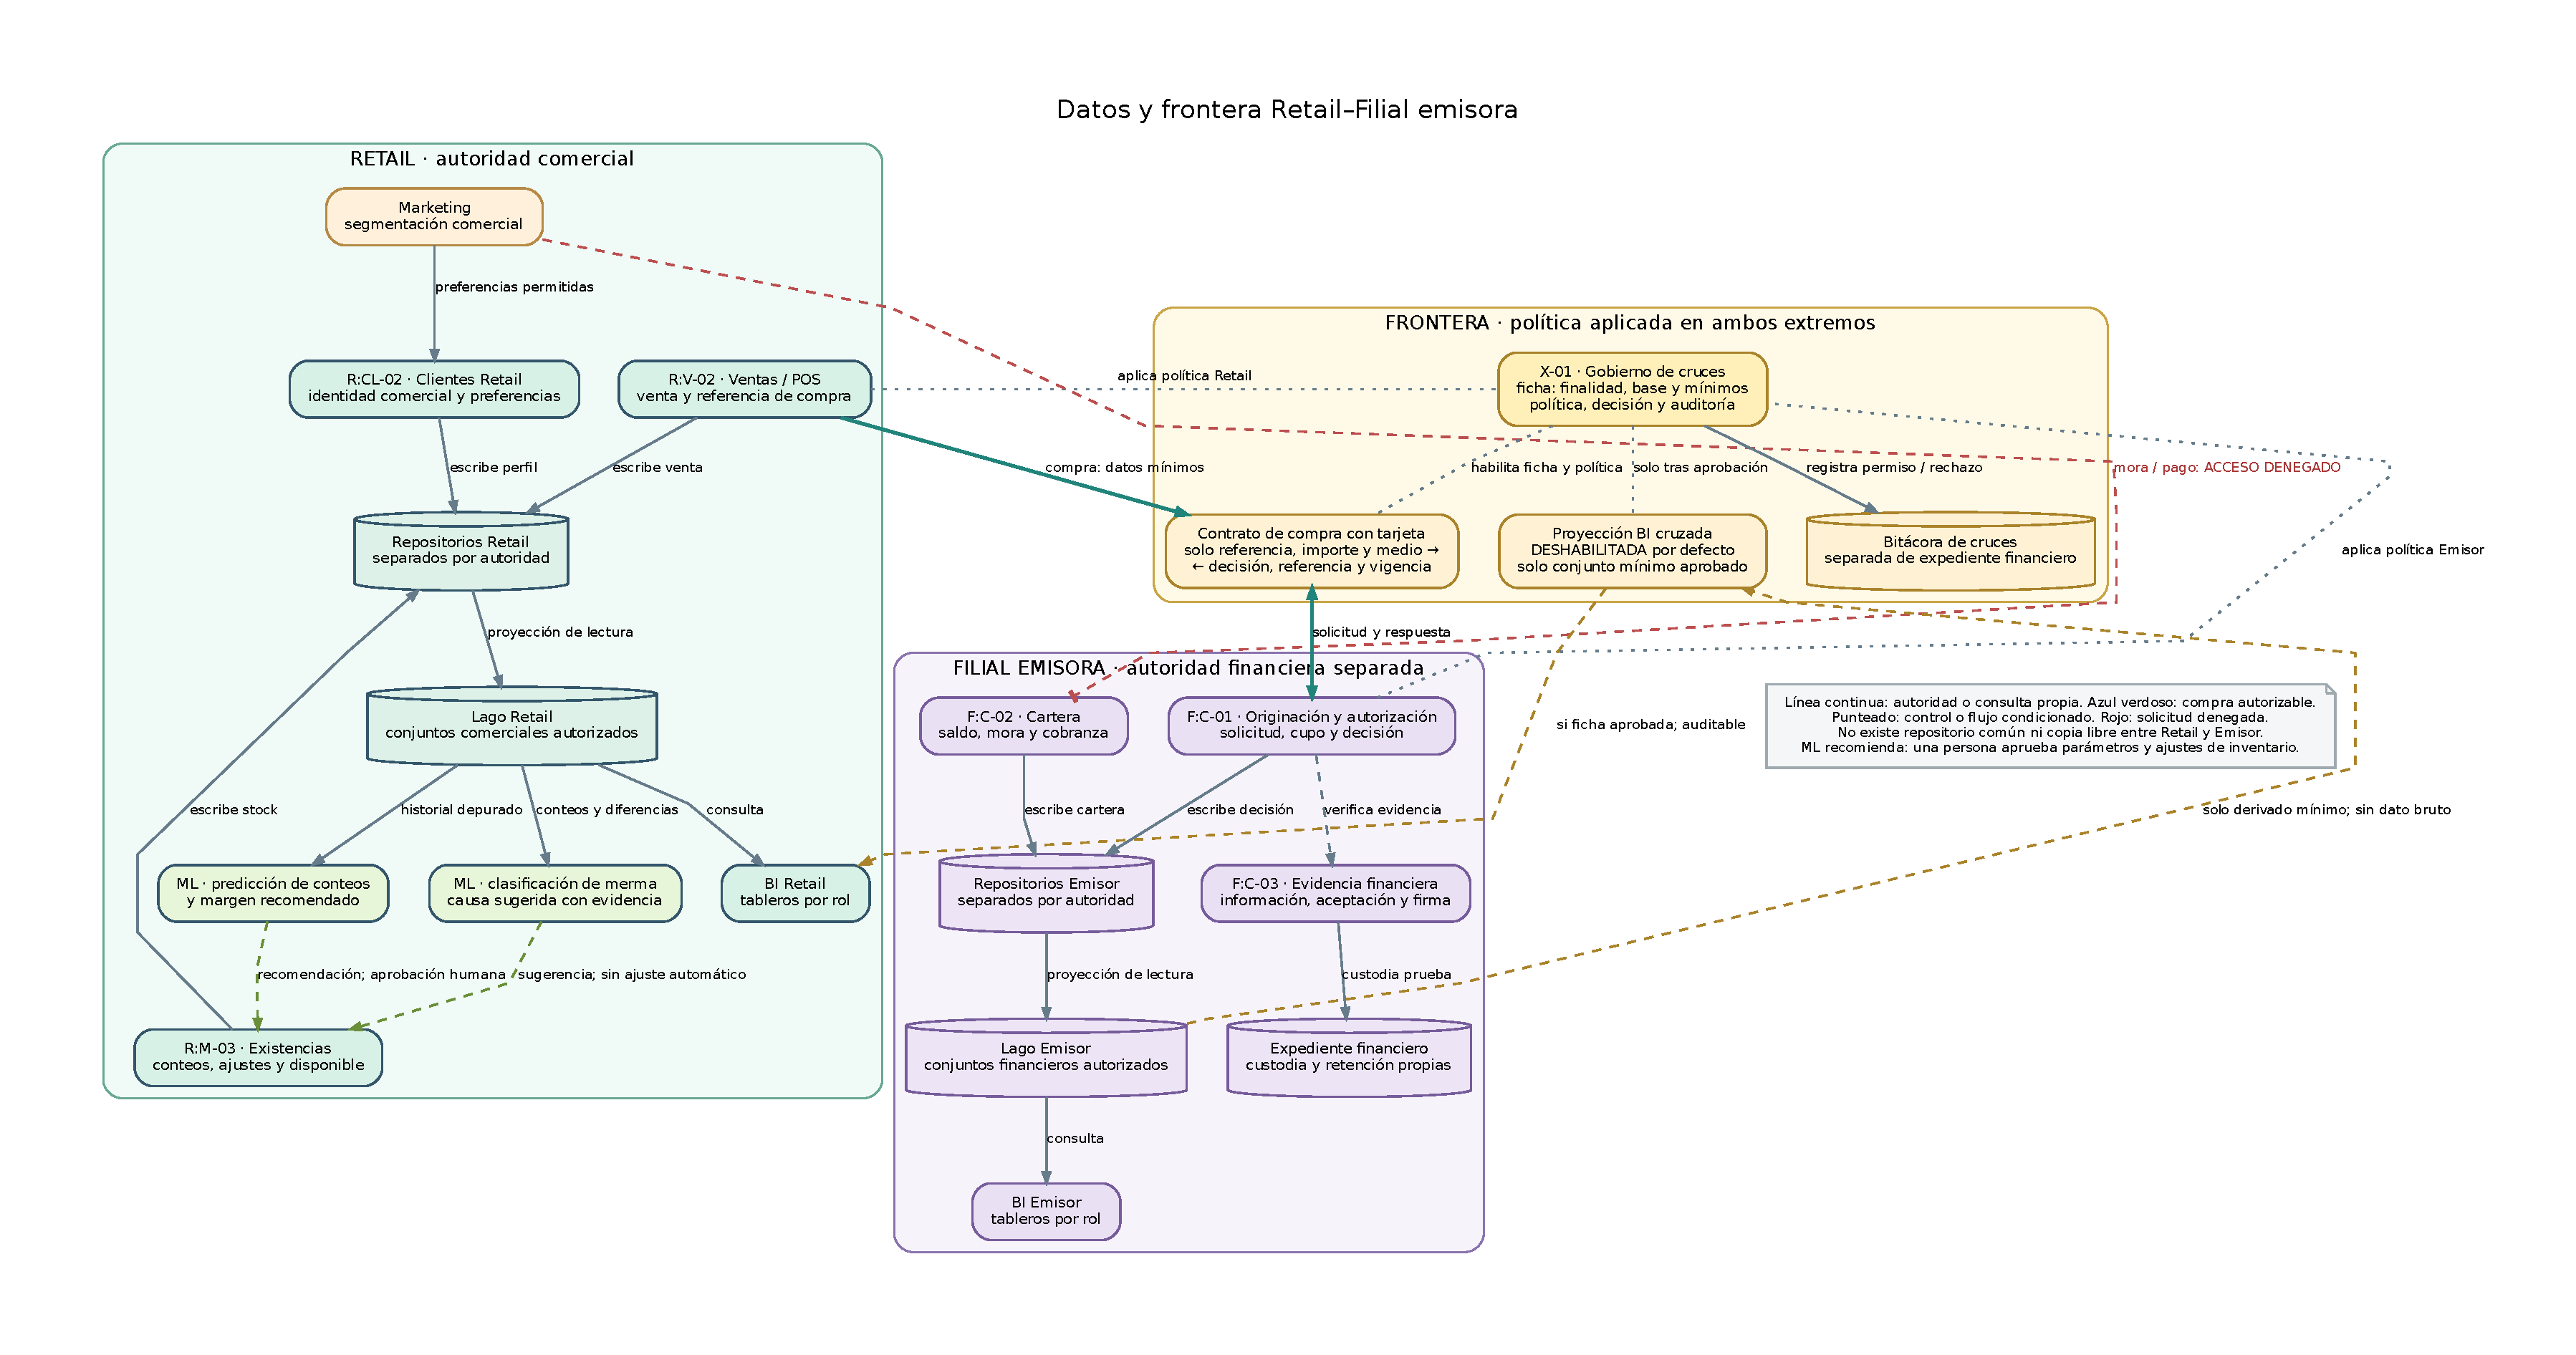
\includegraphics[width=\linewidth]{figuras/diag-04-05_datos-y-frontera.pdf}
\end{center}

Figura 4.5: Autoridades de datos, analítica y frontera Retail--Emisor. Fuente: elaboración propia a partir de SD-03 y RT-02.03.

\subsubsection{Seguridad, continuidad y observabilidad}

Retail y Emisor emplean identidades de servicio, permisos y claves segregados. Los accesos se autorizan por rol, entidad, finalidad y recurso; todo cruce usa el catálogo de X-01 y registra versión de política, decisión, campos liberados y correlación. El tráfico entre servicios y hacia plataformas integradas se cifra; los repositorios cifran datos en reposo. Los registros operativos evitan incorporar saldos o expedientes completos. F:C-03 conserva la evidencia contractual bajo su calendario de retención; la bitácora de X-01 tiene su propia regla jurídica por definir. Las pruebas incluyen una solicitud válida mínima, una ruta no inventariada y un intento de uso secundario rechazado.

El intermediario de eventos separa productores, consumidores, canales, credenciales y permisos de Retail y del Emisor. Un evento financiero no se publica en un canal de Retail; el resultado mínimo de una compra cruza por su contrato aprobado y queda registrado conforme a X-01. Las proyecciones analíticas mantienen espacios de datos y permisos independientes, también para consulta de detalle, exportación e informes programados. La ubicación de un adaptador frente a un sistema conservado se resolverá después de acreditar dónde reside ese sistema y qué conectividad privada admite.

La continuidad local de tienda por 24 horas exige oferta y promociones vigentes, consulta local de existencia, registro durable de ventas y sincronización al restablecer el enlace. El diario local distingue pendiente, enviado, confirmado y en conflicto; registra identificador de operación, tienda y secuencia para que R:V-02 deduplique y reconcilie sin duplicar cobros. La conectividad recuperada no libera una venta pendiente hasta confirmar su recepción y resolver conflictos según una regla documentada. ERP/DTE mantiene la autoridad tributaria: la emisión durante contingencia requiere una modalidad fiscal aprobada y probada, que se especificará en 4.2 y en el procedimiento operativo. Sin enlace no se originan tarjetas ni se amplían cupos. Las compras con crédito previamente autorizado requieren una decisión de riesgo y contrato específicos antes de habilitarse. El piloto prueba corte, operación de 24 horas, retorno y conciliación.

La observabilidad enlaza solicitud, evento y efecto mediante una referencia de correlación sin exponer datos sensibles. Se medirán retraso de publicación de disponibilidad y precio, confirmaciones de reserva, pedidos sin avance, eventos en reintento, diferencias de conciliación, decisiones denegadas por X-01, tiempo de evaluación crediticia y recuperación de evidencias. Las alertas apuntan a la promesa afectada y a su responsable. La memoria de capacidad derivará tasas normales y de evento, almacenamiento y crecimiento del Caso 09 antes de fijar cuotas, particiones o SLO técnicos; la aceptación usa las metas y pruebas de 3.2 y 3.4.

\subsubsection{Decisiones y comprobaciones pendientes}

La Tabla 4.5 reúne las decisiones que rigen el diseño y la prueba que debe sostener cada una. Las alternativas se revisarán con las mediciones del levantamiento antes de cerrar los ADR.

Tabla 4.5: Decisiones de arquitectura y pruebas de validación.

\begin{longtable}{@{}p{0.17\linewidth}p{0.47\linewidth}p{0.27\linewidth}@{}}
\toprule Decisión & Justificación & Verificación \\
\midrule\endhead\bottomrule\endlastfoot
ADR-01: escenario B & Retirar por olas la dependencia del núcleo Retail de 2009, con autoridad por registro. & Mapa de interfaces, conciliación y retorno por ola. \\
ADR-02: datos separados & La tienda y el Emisor responden a regímenes y finalidades distintas. & Pruebas de denegación y auditoría de X-01. \\
ADR-03: contratos mixtos & Respuesta inmediata en pasos bloqueantes; eventos durables para propagación y conciliación. & Latencia, duplicados, reintento y pérdida de enlace. \\
ADR-04: POS local & Sostener la venta de tienda durante interrupción de enlace. & Piloto de 24 horas y retorno sin pérdida ni duplicidad. \\
ADR-05: partición DDD & Separar componentes críticos sin trasladar a microservicios las plataformas conservadas. & Prueba de carga, fallas aisladas y costo de operación. \\
ADR-06: broker y gateway & Publicar hechos confirmados y gobernar la entrada API. & Comparar Kafka, Event Hubs y Service Bus; probar relectura, duplicados, corte regional y contratos de adaptadores. \\
\end{longtable}

Antes de cerrar 4.1 se requieren el inventario de las catorce interfaces, la aprobación jurídica de cada cruce, la política de precio exhibido frente a caja, la regla de resolución de falta de stock posterior a la promesa, la modalidad fiscal de contingencia, la decisión de riesgo para crédito sin enlace, y la memoria de capacidad. Esas decisiones alimentan 4.2, los contratos y los planes de prueba; ninguna debe presentarse como resuelta por un diagrama conceptual.

\subsection{4.1.1 Especificaciones Tecnologías de Software a utilizar}

La Tabla 4.6 propone tecnologías candidatas para las nuevas capacidades. Microsoft Azure queda como referencia preferente, coherente con la alianza prevista en SD-01; la condición de socio o el acuerdo con un socio certificado todavía debe acreditarse según el artículo 34 de las Bases Administrativas. Google Cloud permanece como alternativa técnica por la disponibilidad documentada de Apache Kafka administrado en Santiago. Ninguna de las dos nubes queda adjudicada antes de comparar disponibilidad por producto y región, recuperación, residencia de datos del Emisor, conectividad híbrida y operación. Las plataformas conservadas mantienen su tecnología propia y se integran mediante contratos. La selección final y las versiones que se ofertarán constarán en el Formulario T-11; el contrato de 56 meses exige actualizar componentes durante la operación.

Tabla 4.6: Tecnologías propuestas y comprobación de selección.

\begin{longtable}{@{}p{0.19\linewidth}p{0.32\linewidth}p{0.41\linewidth}@{}}
\toprule Capacidad & Selección inicial & Alternativa y comprobación \\
\midrule\endhead\bottomrule\endlastfoot
Nube & Azure como referencia: Chile Central primaria y Brazil South secundaria. & Comparar con Google Cloud Santiago y São Paulo; comprobar requisitos, residencia, soporte y alianza acreditable. \\
Servicios de aplicación & Java 25 LTS y Spring Boot 4 para APIs y lógica transaccional. & Comparar con otro marco soportado; medir desempeño, competencias y ciclo de actualización. \\
Interfaces nuevas & TypeScript y React para portales y vistas POS. & El modo local y los periféricos del POS requieren prototipo antes de fijar su empaquetado. \\
Microservicios propios & Contenedores en Azure Kubernetes Service (AKS). & Comparar GKE en Google Cloud; validar disponibilidad, aislamiento, escalado y recuperación por región. \\
Eventos & Broker por seleccionar: Kafka es la preferencia, sujeta a costo y prueba de operación híbrida. & Comparar Kafka en AKS o administrado, Event Hubs y Service Bus; probar relectura, errores, orden, recuperación y control por ámbito. \\
Entrada API & Azure API Management como candidato de gateway. & Comparar con Apigee; validar políticas, cuotas, identidad y disponibilidad de nivel de servicio en cada región. \\
Adaptadores & Componentes propios en contenedores o cómputo administrado. & Probar compatibilidad, error y conciliación con cada plataforma conservada. \\
Datos transaccionales & Azure Database for PostgreSQL Flexible Server, con aislamiento por contexto. & Comparar con Cloud SQL; probar alta disponibilidad, replicación y capacidad del nivel escogido. \\
Caché & Caché Redis administrada, solo para datos reconstruibles. & Fijar producto regional tras validar disponibilidad; no almacena autoridad de negocio. \\
Analítica & Azure Data Lake Storage Gen2 y Power BI, con entornos Retail y Emisor separados. & Seleccionar motor analítico tras probar permisos y linaje, considerando que Fabric completo no está disponible en Chile Central y comparando BigQuery y Looker. \\
Identidad y secretos & Federación con directorio del Cliente; Microsoft Entra ID y Key Vault como candidatos. & Confirmar identidad existente y sus protocolos antes de fijar integración. \\
Telemetría & OpenTelemetry y Azure Monitor como candidatos. & Verificar observabilidad conjunta de nube, centro de datos y tiendas. \\
Infraestructura y entrega & Terraform y canal CI/CD con registro de artefactos y despliegue auditado. & Reutilizar canal del Cliente si satisface revisión, firma y trazabilidad. \\
Tienda desconectada & Nodo local redundante con diario transaccional y sincronizador. & Fijar motor y empaquetado tras inventario de hardware, periféricos y ensayo de 24 horas. \\
\end{longtable}

En Azure Chile Central no se ha acreditado aún un servicio administrado de Apache Kafka; Confluent Cloud documenta Azure Brazil South, pero no Chile Central. Operar Kafka en AKS agrega responsabilidad de disponibilidad, actualizaciones y recuperación que debe dimensionarse y probarse. Event Hubs ofrece un punto de conexión compatible con el protocolo Kafka, pero no equivale al broker Apache Kafka; Service Bus ofrece colas y tópicos con semántica diferente. La comparación decidirá qué propiedades necesita cada flujo antes de elegir producto. La región primaria y la secundaria necesitan procedimientos explícitos de replicación y conmutación. Ningún broker confirma reservas ni decisiones crediticias en línea. La disponibilidad publicada y el resultado de una compra dependen de contratos síncronos con límites de espera. Los modelos predictivos de conteo y merma ejecutarán entrenamiento e inferencia como apoyo separado de la escritura de existencias, con trazabilidad y supervisión conforme a RT-18.

\section{4.2 Arquitectura física}

La carga principal de la solución nueva se plantea en nube pública, con Azure como referencia para el diseño físico y Google Cloud como alternativa por comparar. Se conserva operación local en tiendas y conexión al centro de datos actual mientras permanezcan dependencias heredadas. La Tabla 4.7 ubica componentes nuevos sin asignar a una ubicación inventada los sistemas existentes. La configuración de los ambientes de Desarrollo, QA, Preproducción, Producción y Recuperación ante Desastres se definirá como código; las pruebas de Preproducción y de recuperación usarán las mismas clases de componentes y las capacidades exigidas por las Bases, ajustadas a su finalidad. La red separa borde público, aplicación y datos privados, y conecta el sitio del Cliente por enlaces redundantes conforme a RT-03.17.

Tabla 4.7: Emplazamiento inicial de los componentes de la solución.

\begin{longtable}{@{}p{0.30\linewidth}p{0.26\linewidth}p{0.36\linewidth}@{}}
\toprule Componente lógico & Emplazamiento propuesto & Condición de diseño \\
\midrule\endhead\bottomrule\endlastfoot
Borde, gateway y servicios propios & Región primaria Santiago; recuperación en São Paulo. & Dos zonas para cargas críticas; acceso privado a aplicación y datos. \\
Broker de eventos y repositorios transaccionales & Santiago con alta disponibilidad; réplica de recuperación en São Paulo. & Producto por seleccionar, RPO y RTO por servicio, réplica probada y autorización de residencia. \\
Analítica Retail y Emisor & Proyectos y almacenamiento separados en la nube. & Permisos y claves por entidad; cruce solo por contrato aprobado. \\
POS y diario de contingencia & Terminal y nodo local redundante en cada tienda. & Operación de 24 horas, disco tolerante a falla y retorno conciliado. \\
Adaptadores a sistemas conservados & Nube o centro de datos según interfaz y ubicación comprobadas. & No fijar ruta ni latencia antes de levantar las catorce interfaces. \\
ERP/DTE, WMS y marketplace & Permanecen en sus plataformas actuales. & Alojamiento individual y conectividad por verificar. \\
Comercio electrónico y fidelización & Permanecen integrados durante la evaluación. & Conservación o sustitución condicionada a pruebas de primera etapa. \\
\end{longtable}

La Tabla 4.8 reúne los emplazamientos y las comprobaciones que deben pasar al diseño físico. Una ruta propuesta no acredita que el enlace exista hoy.

Tabla 4.8: Nodos y comprobaciones para el diseño físico.

\begin{longtable}{@{}p{0.14\linewidth}p{0.37\linewidth}p{0.41\linewidth}@{}}
\toprule Nodo & Función y autoridad & Comprobación antes de fijar topología \\
\midrule\endhead\bottomrule\endlastfoot
SIT-01 & 22 tiendas, POS, periféricos, diario y sincronización local. & Inventario por tienda, dos enlaces donde aplique, 24 horas de continuidad y retorno. \\
CD-01 & Distribución principal; operación física con WMS conservado. & Equipos, red y ubicación real del servidor WMS. \\
CD-02 & Distribución Concepción; operación logística con enlace actual único. & Redundancia de enlace, funcionalidad requerida y eventual extensión WMS. \\
DC-01 & Centro de datos de casa matriz, 140 m², compartido por Retail y Emisor. & Inventario de las plataformas allí alojadas, brechas físicas y enlaces a nube. \\
DC-02 & Sala de respaldo del Cliente en la misma comuna. & Capacidad, dependencias comunes con DC-01 y función real en recuperación. \\
CLD-01 & Región primaria propuesta: aplicación, broker, datos y analítica segregados. & Zona, producto disponible, redes privadas, residencia, capacidad y operación. \\
CLD-02 & Región secundaria propuesta para recuperación de cargas nuevas. & Réplica por dato, aprobación jurídica, RTO/RPO y conmutación ensayada. \\
EXT-01 & Transportistas, medios de pago, marketplace y proveedores. & Contrato, protocolo, ubicación y frontera de cada contraparte. \\
\end{longtable}

Cada arista del diagrama físico tendrá origen, destino, contrato, dirección, red, protección, volumen, latencia, responsable y condición de fallo. Esto incluye SIT-01--CLD-01 para sincronización, CLD-01--DC-01 para plataformas que se compruebe alojadas allí, CD-01/CD-02--CLD-01 para operación logística y CLD-01--CLD-02 para recuperación. La ruta hacia una plataforma externa podrá terminar en EXT-01 si el inventario confirma que reside fuera del centro de datos. No se convierte una arista funcional en un enlace físico confirmado sin ese inventario.

El dimensionamiento derivará transacciones normales y de evento, concurrencia, tamaños de mensajes, retención y crecimiento de las cifras del Caso 09. Se medirán reserva y venta de extremo a extremo, retraso de publicación de disponibilidad y precio, atraso de consumidores del broker y sincronización de tiendas. Estas mediciones determinarán réplicas, cuotas, particiones o colas, almacenamiento, enlaces y costo. La dependencia del ERP/DTE para emisión, del WMS para ejecución física y de las plataformas conservadas tendrá un procedimiento de degradación y conciliación por interfaz.

\subsection{4.2.1 Especificaciones Implementos a proveer (Hardware y Software)}

El Formulario T-11 detallará cantidad, versión, licenciamiento, soporte y ubicación de los implementos seleccionados. La especificación de nodos locales, terminales y periféricos se completará con el inventario de las 22 tiendas y el ensayo de continuidad; los equipos, obras y enlaces a cargo del Cliente se distinguirán de la instalación, configuración y certificación a cargo del proponente. No se atribuirá a los nuevos microservicios el hardware ni las licencias de ERP/DTE, WMS, marketplace y demás plataformas conservadas.

\section{4.3 Data center}

La solución híbrida utiliza la nube para la carga principal y las instalaciones del Cliente para la continuidad local y las dependencias que así se acrediten. El recinto propio de casa matriz mide 140 m² y dispone de una sala de respaldo en la misma comuna; el Caso informa una brecha de estándares documentada en un informe interno de 2024 aún no entregado. Esa evidencia y la ubicación real de cada plataforma se incorporarán a la tabla de emplazamiento antes de aprobar el diseño físico.

\subsection{4.3.1 Especificaciones Data Center Primaria}

Para la solución nueva se propone Santiago, región Azure \texttt{chilecentral} como referencia, con servicios críticos distribuidos al menos en dos zonas cuando el producto y nivel elegidos lo admitan, y redes privadas para aplicación y datos. El centro de datos de casa matriz continuará atendiendo los sistemas que efectivamente residan allí durante la convivencia; su función, energía, red, seguridad física y enlaces deberán validarse con el informe de brechas y el inventario. La ubicación de una plataforma conservada no se deduce de que se conecte por un adaptador.

\subsection{4.3.2 Especificaciones Data Center Secundario}

Se propone São Paulo, región Azure \texttt{brazilsouth} como referencia para recuperar los componentes nuevos, sujeto a aprobación jurídica de la residencia y réplica de cada conjunto de datos, especialmente los del Emisor. Chile Central no posee una región emparejada automática; la réplica hacia Brazil South requiere diseño y pruebas por componente. La modalidad inicial será activo-pasivo con conmutación ensayada; para servicios críticos se verificará RTO no superior a cuatro horas y RPO no superior a quince minutos, conforme a RT-07.04. Se probará la conmutación al menos dos veces por año. La sala de respaldo existente en la misma comuna no se supondrá suficiente como única recuperación antes de evaluar su riesgo común con el centro principal.

\section*{Referencias}
\addcontentsline{toc}{section}{Referencias}

Multitiendas Ancoa S.A. (2026a). \textit{Bases administrativas para la preparación de la propuesta} (Licitación N.° TFEP-01/2026, versión 1.0).

Multitiendas Ancoa S.A. (2026b). \textit{Bases técnicas. Caso 09: Cadena multitienda} (Licitación N.° TFEP-01/2026, versión 1.0).

Multitiendas Ancoa S.A. (2026c). \textit{Bases técnicas transversales} (Licitación N.° TFEP-01/2026, versión 1.0).

Only Simple Solutions. \textit{SD-03: Esquema de solución y alcance}, secciones 3.1 a 3.4, revisión de trabajo.

Microsoft. (2026). \textit{List of Azure regions}. \url{https://learn.microsoft.com/azure/reliability/regions-list}.

Microsoft. (2026). \textit{Fabric region availability}. \url{https://learn.microsoft.com/fabric/admin/region-availability}.

Microsoft. (2026). \textit{Azure Event Hubs for Apache Kafka: frequently asked questions}. \url{https://learn.microsoft.com/azure/event-hubs/apache-kafka-frequently-asked-questions}.

Confluent. (2026). \textit{Confluent Cloud regions and availability by cloud provider}. \url{https://docs.confluent.io/cloud/current/get-started/regions.html}.

Google Cloud. (2026). \textit{Managed Service for Apache Kafka locations}. \url{https://docs.cloud.google.com/managed-service-for-apache-kafka/docs/locations}.

Spring. (2025). \textit{Spring Boot 4.0.0 available now}. \url{https://spring.io/blog/2025/11/20/spring-boot-4-0-0-available-now/}.

Oracle. (2026). \textit{Java SE Support Roadmap}. \url{https://www.oracle.com/java/technologies/java-se-support-roadmap.html}.

\section*{Declaración de uso de IA}
\addcontentsline{toc}{section}{Declaración de uso de IA}

Esta versión preliminar de la sección 4.1 se redactó con asistencia de un modelo de lenguaje a partir de las Bases, el alcance y el documento de revisión suministrado por el equipo. Se revisó su estilo con la guía humanizer del proyecto, sin alterar cifras, nombres ni decisiones. Sus afirmaciones requieren validación de los responsables de arquitectura, negocio y cumplimiento antes de la entrega final.

\ossFinalPage
\end{document}
